% !TeX root = ../../main.tex
\section{Process description}

Nitroma's process for the nitration of toluene and subsequent reduction and hydrogenation of nitrotoluenes is unique in both its continuous operating mode and the production of three different substituted aromatic amines.  \Cref{fig:routes-SI} is a summary of the synthesis routes selected by for Nitroma's process.
\begin{figure}[H]
    \centering
    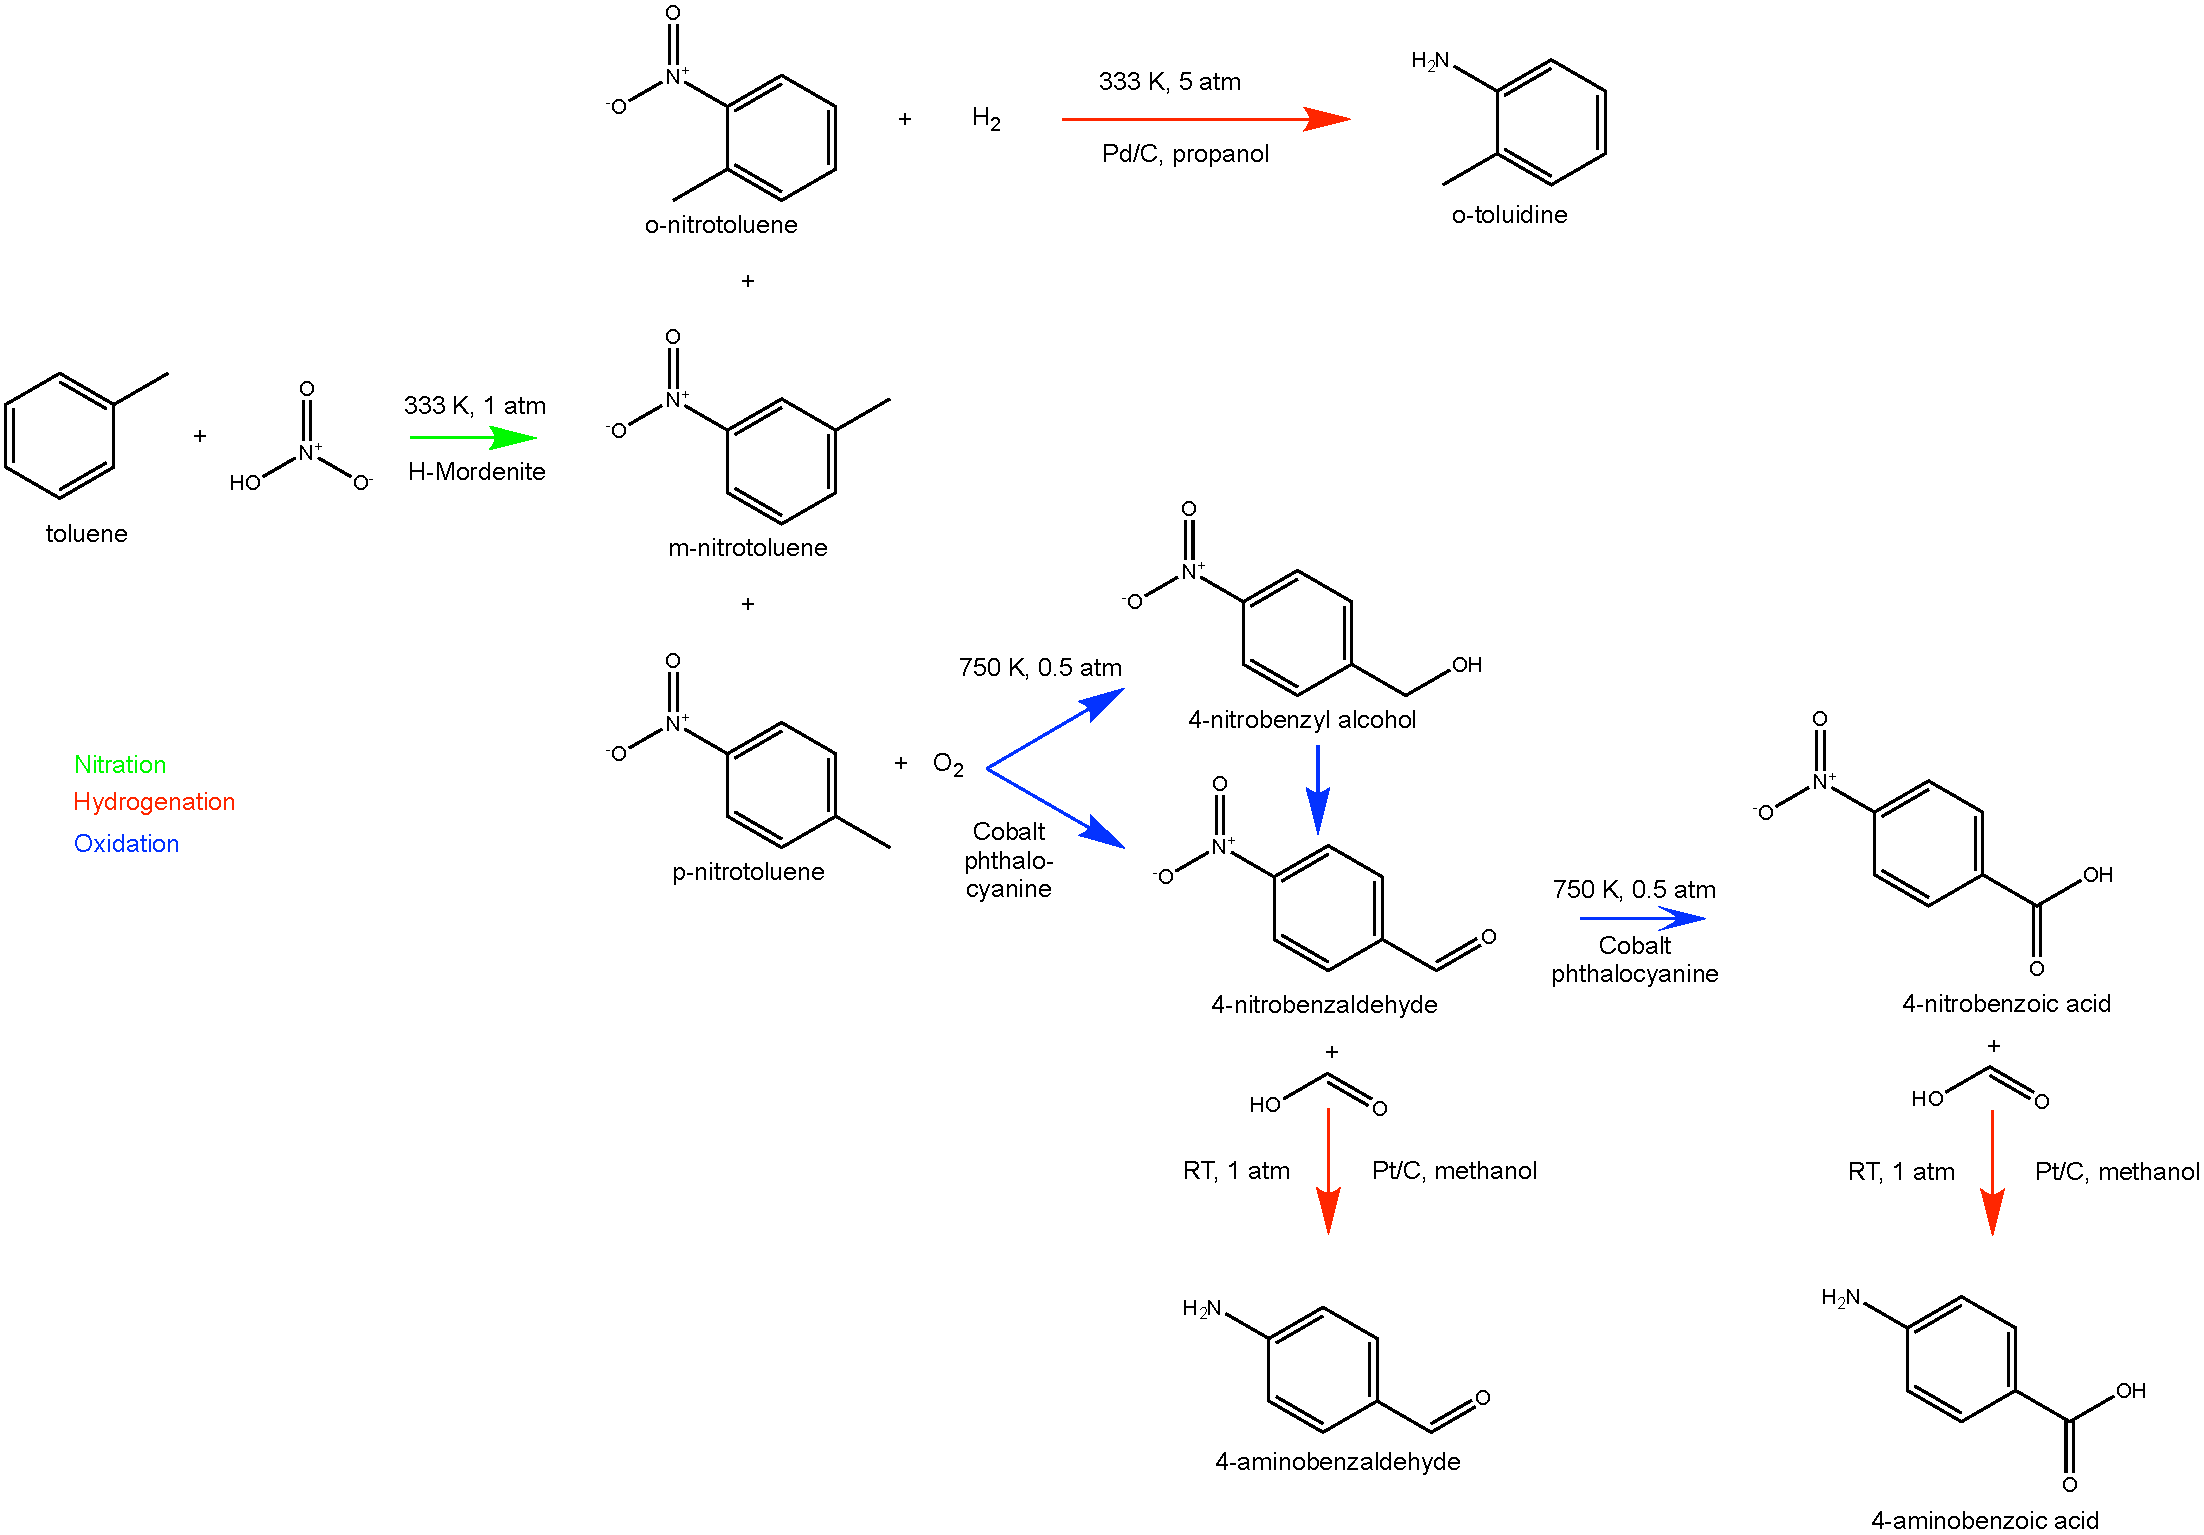
\includegraphics[width=0.8\linewidth]{chapters/2-reaction/figures/routes-chosen.pdf}
    \caption{Synthesis route for Nitroma's process}
    \label{fig:routes-SI}
\end{figure}

Firstly, the nitration of toluene with \SI{70}{\percent} aqueous nitric acid is carried out in a shell-and-tube heat exchanger reactor (R101) packed with H-mordenite catalyst. 1670 tonnes per year of \SI{95}{\percent} pure liquid toluene is mixed (M101) with nitric acid in a 1:2 molar ratio. The reaction takes place at \SI{1.3}{\bar} and the temperature is controlled to stay between \SIlist{325;360}{\K} thanks to an innovative cooling system integrated to the reactor. Conversions above \SI{98}{\percent} can thus be achieved. The solid acid catalyst and the reaction condition favour the more economically desirable \para-nitrotoluene (PNT) isomer. The nitration reactor effluent is fed to a decanter (S101) to separate the aqueous nitric acid from the organic phase. Following water evaporation in a distillation column (S105), nitric acid is recycled back into the nitration reactor at a \SI{99.8}{\mol\percent} purity.  Meanwhile, the organic phase is sent to a distillation column (S102) to recycle unreacted toluene to the nitration reactor. The nitrotoluenes are sent to a second distillation column (S103) to separate the more volatile \ortho-nitrotoluene (ONT) from \meta-nitrotoluene (MNT) and PNT. The large difference in the PNT and MNT melting points is exploited in a mixed-suspension mixed-product removal crystalliser (S104). The solid PNT crystals are then melt in a hydraulic wash column (S106).

Liquid ONT is mixed with methanol (M201) and hydrogenated under pressure over Pd/C catalyst to \ortho-toluidine (o-TOL) in a co-current trickle bed reactor operating with both gas and liquid in downflow mode. Trickle bed reactor (R201) is chosen due to the ease of operation at high pressure and the relative slow catalyst deactivation. The reactor is operated at \SI{333}{\K} and \SI{5}{\atm} to achieve conversions over \SI{95}{\percent}. o-TOL is then purified to achieved a purity of \SI{99.4}{\mol\percent}. The hydrogen gas leaves the reactor via an outlet port and his recycled by. The liquid effluent enters a distillation column (S201) to separate methanol and water from the less volatile organic compounds. Methanol is further distilled (S203) to be recycled to the reactor. Unreacted ONT is recycled back to the reactor following stripping (S202) from the o-TOL. The purified o-TOL is cooled down with air and is granulated (G201) before packaging and storage.

Meanwhile, gaseous PNT is fed into an air-oxidation reactor (R301) packed with cobalt phthalocyanine catalyst to be partially oxidised to 4-nitrobenzaldehyde (4-NBH). Depending on the production campaign, the reactor effluent can either be sent to a second oxidation reactor (R401) where 4-NBH and unreacted PNT will be completely oxidised to 4-nitrobenzoic acid (4-NBA), owing to longer residence times; or directly to a liquid-phase hydrogenation reactor (R501). Ultimately, 4-NBH and 4-NBA are both reduced to respectively 4-aminobenzaldehyde (4-ABH) and 4-aminobenzoic acid (4-ABA) with formic acid diluted in a methanol solvent over Pt/C catalyst. The effluent from the partial oxidation reactor is flashed (S301) and decanted (S302) to remove excess gas before the separation of PNT to be recycled (S303). 

In the 4-ABH campaign, the bottom outlet of S303 is sent to another distillation column (S501) to separated 4-NBH from the inevitable complete oxidation product 4-NBA. The effluent from R501 is flashed (S502) and sent to two distillation columns: the first one to recover unreacted 4-NBH (S503) and the second one to purify 4-ABH (S504) which is then cooled down and granulated (G501) before packaging and storage.  
In the 4-ABA campaign, the bottom outlet of S303 is sent R401 whose effluent is flashed (S401) and then mixed with methanol and formic acid for reduction in R601. 4-ABA is finally recovered as a solid following  crystallisation in a continuous falling-film melt crystalliser (S601).

To meet the current customer demand, Nitroma's plant operates a 240-day 4-aminobenzaldehyde campaign and a 35-day 4-aminobenzoic acid campain, thus yielding \SI{652}{\tonne\per\year} of \SI{99}{\percent} pure \ortho-toluidine, \SI{538}{\tonne\per\year} of \SI{99.3}{\percent} pure 4-aminobenzaldehyde and \SI{100}{\tonne\per\year} of pure 4-aminobenzoic acid.

The waste produced by Nitroma's process is treated on-site in waste treatment units designed to accommodate unreacted organic substances, spent nitric acid and methanol that could not be recovered via recycling. The spent nitric acid is directly sent to a neutralisation unit to treat it with lime. Following filtration, the solid deposits will be sent to landfill while the filtrate is mixed with the other waste streams. All liquid waste streams are treated first by adsorption using activated carbon followed by treatment in an anaerobic membrane bioreactor (AnMBR). Collaboratively, the use adsorption and AnMBR reduces the overall chemical oxygen demand of the liquid waste effluent below the maximum limit of \SI{250}{\mg\per\litre}. Meanwhile, the gaseous waste streams containing organic compounds are disposed of via incineration in a low \ch{NO_x} burner before being passed through a wet scrubber to limit emissions of greenhouse gases.
